
\documentclass[10pt]{article}

\usepackage{amsmath,amssymb,amsthm}
\usepackage{booktabs}
\usepackage{color}
\usepackage{enumitem}
\usepackage{fullpage}
\usepackage{graphicx}
\usepackage[hidelinks]{hyperref}
\usepackage[utf8]{inputenc}
\usepackage{multirow}
\usepackage{tikz}
\usetikzlibrary{automata,positioning}
\usepackage{float}
\usepackage{listings}
\usepackage{tikz}
\usepackage{amsmath}
\usetikzlibrary{shapes,arrows,positioning}
\usepackage{vmargin}
\usepackage{algorithm}
\usepackage{algorithmic}
\usepackage{cancel}
\usepackage{mathtools}


\DeclarePairedDelimiter\ceil{\lceil}{\rceil}


\hypersetup{pdfstartview = FitH} %hace que la hoja se expanda en anchura, y no se muestre toda la hoja al abrirlo

\addtolength{\textwidth}{0.5in} % a=2b
\addtolength{\hoffset}{-0.45in} % -b
\addtolength{\textheight}{0.9in} % c
\addtolength{\voffset}{-0.4in} % -c

\renewcommand{\labelenumi}{(\alph{enumi})}
\newcommand{\pt}[1]{{\bf ({#1} puntos)}}
\newcommand{\euler}{e}

\parskip 1ex
\parindent 0ex

\allowdisplaybreaks

\pagestyle{empty}
\begin{document}

\begin{tabular}{ l l }
  \multirow{1}{*}
  {
\includegraphics[height=1.2in]{logo uc.png}}
  & \textsc{Pontificia Universidad Católica de Chile} \\
  & \textsc{Escuela de Ingeniería} \\
  & \textsc{Departamento de Ingeniería Industrial y de Sistemas} \\
  & \textsc{ICS2122 -- Taller de Investigación Operativa} \\
  & \textsc{Profesores: Gonzalo Pérez, Marcelo Pérez, Ariel Espinoza, Matías De Geyter,} \\
  & \textsc{Elbio Avanzini, Alejandro Mac Cawley} \\
  & \textsc{Ayudante jefe: Francisco Tamarín} \\
  & \textsc{Segundo Semestre 2023} \\
\end{tabular}

\vspace{20mm}

\begin{center}
\LARGE
\textbf{Informe 1}
\end{center}
\rule{16cm}{0.1mm}

\begin{center}
    \Large\textbf{Mantenimiento predictivo mediante datos categóricos de una línea de embotellado}
\end{center}
\rule{16cm}{0.1mm}
\begin{center}
    \Large\textbf{Grupo 5}
\end{center}
\vspace*{80mm}
\begin{flushright} % Alineación a la derecha
\begin{tabular}{ r r }
  & \textsc{Tomás Arancibia} \\
  & \textsc{Consuelo Honorato} \\
  & \textsc{Florencia Lira} \\
  & \textsc{Antonia Orrego} \\
  & \textsc{Rafaela Rámirez} \\
  & \textsc{Macarena Tagle} \\
  & \textsc{Gaspar Villarroel} \\
\end{tabular}
\end{flushright}

\newpage
\renewcommand{\contentsname}{Índice}
\tableofcontents
\newpage
\section{Resumen}
En el presente informe se desarrolla un análisis detallado sobre el trabajo de investigación realizado con la línea de embotellamiento de vinos de una empresa vitivinícola. El objetivo es actualizar las políticas de mantenimientos ya existentes, pasando de uno preventivo/correctivo hacia uno predictivo, el cual busca mejorar la eficiencia operativa y la gestión del mantenimiento de la máquina automatizada, así optimizando al máximo las utilidades y recursos de la empresa. El proyecto está sustentado en datos de tipo categóricos, los cuales están presentes en cuatro bases de datos distintas: avisos, alarmas, mantenciones y producción. Estas contienen información de distintas ocurrencias en un periodo de 20 meses, juntando entre ellas mas de 4 millones de observaciones. Gracias a la investigación de las bases de datos en conjunto, se pudo analizar el comportamiento de las ocurrencias de la maquinaria con respecto a las mantenciones realizadas, y se pudo concluir que la manera en que se actuaba no resultaba beneficioso para la linea de embotellado otorgándole el valor e importancia de resolver el problema debido a las pérdidas económicas que esto puede causar pensando en los recursos limitados con los que cuenta la empresa. Además, a partir de ellas se establecen metas a cumplir e indicadores que permitan medir el desempeño, así dar cuenta del impacto de las metodologías de modelos predictivos en la eficiencia de la línea. Se utilizará un enfoque 50/25/25, para dividir los datos en entrenamiento, validación y pruebas. Para ello, se analizan y discuten distintas metodologías encontradas en la literatura, incluyendo las redes neuronales recurrentes, métodos de suavización exponencial, método Holt-Winter, método de Croston y SBA y Fast Fourier Transform. Se pudo investigar sobre fortalezas y debilidades de cada metodología, para tener un acercamiento real a como se extrapolaría cada método al problema de la línea de embotellado y su predicción de fallas y luego se realizó un análisis comparativo tomando en cuenta los puntos claves para elegir la metodología que se adapta mejor a la resolución de la problemática poniendo énfasis en la complejidad y tamaño de los datos, parámetros a estimar y variables endógenas y exógenas. 



\section{Introducción}

En el entorno de los procesos productivos empresariales, la optimización y agilización de la producción son pilares fundamentales para satisfacer la demanda y alcanzar una máxima rentabilidad. Sin embargo, estos objetivos pueden verse amenazados por las incidencias en los recursos operacionales, específicamente en la maquinaria responsable de los procesos de la empresa, lo que impulsa la necesidad de una aproximación mas exacta a los momentos en que se requiere de un mantenimiento, y así disminuir los periodos de inoperancia. \\
\\
Los sistemas de embotellado, con su maquinaria especializada y ritmo constante, están sometidos a un desgaste que puede llevar a fallas costosas y tiempos de inactividad no planificados, que pueden significar el no cumplimiento de la demanda. Si se cuenta con un sistema de mantenimiento correctivo o preventivo, como es el caso de la empresa en cuestión, no se está abordando de manera óptima las fallas imprevistas y los recursos, lo que puede resultar en tiempos de inactividad y gastos innecesarios y falta de capacidad para prever y evitar problemas críticos de manera anticipada. En la actualidad, numerosas organizaciones están optando por estrategias de mantenimiento predictivo por una serie de razones fundamentadas. El enfoque de mantenimiento predictivo se basa en la utilización de datos históricos y técnicas de análisis para prever posibles fallos en la maquinaria antes de que ocurran. Además de prolongar la vida útil de los equipos, es una herramienta esencial para prevenir las interrupciones no planificadas, reducir costos operativos y garantizar un óptimo funcionamiento que conlleve a una mayor seguridad en los procesos productivos. \\
\\
Ahora se cuenta con el desafío de desarrollar una metodología de mantenimiento predictivo para la línea de embotellamiento de una empresa vitivinícola, cuyo nombre aun no se sabe. Para lograrlo, se cuenta con bases de datos que contienen un gran volumen de información registrada en los últimos veinte meses. Esta tarea implica la aplicación de algoritmos y modelos avanzados de análisis de datos para identificar patrones, tendencias y señales tempranas de problemas o anomalías. A medida que se avanza en la investigación, se cree que el enfoque en el mantenimiento predictivo ofrecerá beneficios significativos para la empresa y contribuirá al éxito continuo de la línea de embotellamiento en este mercado altamente competitivo. En las secciones siguientes de este informe, se detallan los pasos que se han seguido y los que quedan por cumplir, con el objetivo de proporcionar una visión completa del trabajo realizado y sus implicaciones para el proceso de embotellamiento.


\section{Descripción del problema}

\subsection{Antecedentes}

Una línea de embotellamiento de vinos consta de 4 etapas; enjuague, lavado y secado, llenado y tapas. Siguiendo un proceso de Monoblock en una máquina automatizada, con una serie de estaciones con eventos y operaciones de manera secuencial. Cada evento presente en un proceso de embotellamiento en empresas vitivinícolas, es de suma importancia para lograr un procedimiento eficiente y eficaz. Es por esto que es necesario analizar cada una de estas y cómo afectan a la producción cuando se generan distintos tipos de fallas.  \\
\\
Actualmente, esta empresa hace uso de un modelo de mantenimientos preventivos el cual se basa en hacer mantenimientos periódicos antes de que ocurra la falla, por lo que, al no ocupar el 100${\%}$ de la capacidad de la máquina, se crea un costo adicional considerable en la utilidad de la empresa. Además, en caso de que la máquina presente una falla imprevista, la embotelladora toma una postura correctiva, realizando una mantención a producción cero, afectando directamente los volúmenes productivos de la empresa. Esto trae consigo bastantes consecuencias perjudiciales en la eficiencia operativa de la línea de embotellamiento. Si bien, se reduce el riesgo de fallas inesperadas, los recursos son limitados, por ende, esto puede generar costos de recursos y utilidades donde no son estrictamente necesarios. El modelo correctivo, por otro lado, detiene la línea de producción dificultando la capacidad de satisfacer la demanda del mercado en el tiempo solicitado. \\
\\
La detección y gestión de defectos es crucial en el ámbito del correcto funcionamiento de la línea productiva, debido a las enormes pérdidas económicas y de recursos que pueden generar, incluso si algunos de esos defectos resultan ser falsas alarmas. Existe un claro trade-off entre las tres metodologías de mantenimiento mencionadas con anterioridad. Por un lado, el mantenimiento correctivo implica abordar las fallas una vez que se detectan, lo que puede ser costoso y peligroso si la detección es tardía. Por otro lado, el mantenimiento preventivo se basa en programar revisiones periódicas de componentes en función de su edad, lo que puede ser efectivo en casos donde la probabilidad de falla está relacionada con la edad del equipo, pero puede llevar a un mantenimiento repetitivo e innecesario en otros casos.\\
\\
Para superar estas limitaciones y anticipar defectos mientras se evitan mantenimientos innecesarios, se introduce el mantenimiento predictivo. Esta metodología se basa en datos en tiempo real y datos históricos para estudiar y comprender las causas de los defectos. El objetivo es identificar las condiciones que generan defectos y, si los resultados son prometedores, se busca encontrar el equilibrio entre la detección temprana de defectos y la minimización de mantenimientos innecesarios en la maquinaria (Lopez, 2021).\\
\\
La empresa vitivinícola en cuestión cuenta con una gran recopilación de datos ordenados, tanto categóricos como continuos, que ha utilizado para optimizar su operación en la línea de embotellamiento. Para esto, es necesario también hacer cuenta de los mantenimientos que se deben realizar, y minimizar su ocurrencia, ya que estos significan detener la producción. Al observar los datos entregados, los mantenimientos que se realizan no cuentan con ningún tipo de periodicidad definida, por lo que es necesario definir un mantenimiento predictivo en base a la información entregada, con el fin de contar con un modelo proactivo de mantención en base a las necesidades específicas según las condiciones del contexto operativo y así maximizar la productividad en la línea.

\subsection{Exploración de datos}

Para el análisis de datos se dispuso de 4 bases de datos. Algunos elementos comunes que poseen estas bases de datos es el registro temporal el cual al hacerlas coincidir definen el marco temporal de estudio desde el 06/09/2022 hasta el 14/06/2023, es importante mencionar que se esta trabajando con una maquina en especifico de la marca ``Bertolaso'', por lo que la gran mayoría de los datos son generados por ella o se encuentran relacionados a ella. Los únicos datos que no son obtenidos directamente de la máquina son las fechas de las mantenciones, las cuales fueron proporcionadas directamente por la empresa.\\

A continuación se detallan cada una de las bases de datos:\\

\textbf{Alarmas}: Esta base de datos corresponde a información entregada por la máquina que muestra la ocurrencia de estos eventos denominados alarmas en varios instantes de tiempo, este tipo de evento se caracteriza por mostrar un cambio en el comportamiento de la maquina que debe ser considerado según su gravedad, ya que se registran desde ocurrencias de rutina hasta  fallas que significan su mal funcionamiento. Esta posee una longitud de 14,952 observaciones, de las cuales se logro extraer un total de 81 alarmas distintas, las cuales se encuentran detalladas en el Anexo (). En particular esta base posee una columna denominada causa la cual clasifica las alarmas en 6 tipos : "No Asignado", "Generic Cause", "Internal Cause","External Cause","Operator Action","Outfeed Accumulation"\\

\textbf{Avisos}: Esta base de datos sigue el mismo comportamiento que la base de alarmas, es un registro en el tiempo de la ocurrencia de eventos que se catalogan como avisos. Su longitud es de 199,287 observaciones, debido a la 
se distinguieron 49 tipos de avisos distintos que se encuentran detallados en el Anexo (), debido a las descripciones y la frecuencia con que ocurren demuestran que la gravedad de los avisos es menor a de las alarmas.\\

\textbf{Mantenciones}: Contiene un registro de las mantenciones realizadas por la empresa, con la especificación de la duración y fecha realizada. Se cuentan con 13 instancias de mantención, de las cuales solo 7 son efectivas para el análisis ya que pertenecen al marco temporal. De las fechas se extrae que estas no se realizan de forma periodica, ocurriendo en intervalos de tiempos variables entre una y otra.\\

\textbf{Producción}: Con una longitud de 3,676,125 observaciones, esta base de datos muestra los ritmos de producción registrados por la maquina a lo largo del tiempo. \\

Tanto la base de datos como la avisos seguía un patrón de registro el cual consiste en escribir horizontalmente la ocurrencia de varios eventos que ocurrieron en un intervalo de tiempo, cada una de ellas podia registrar hasta 10 eventos. Con el propósito de individualizar las ocurrencias se genero una nueva base de datos con un registro vertical, incluyendo las siguientes variables:

\begin{itemize}
\item \textbf{UNIX\_T}: El "tiempo Unix" o "marca de tiempo Unix" se refiere a una forma particular de representar el tiempo en sistemas operativos tipo Unix, como Linux. En esta representación, el tiempo se mide en segundos transcurridos desde un punto de referencia específico conocido como el "epoch" o "época" de Unix. El "epoch" de Unix es el 1 de enero de 1970 a las 00:00:00 UTC (Tiempo Universal Coordinado).
\item \textbf{Tipo}: Esta variable fue creada al juntar las dos bases de datos para indicar si la ocurrencia de la fila corresponde a una Alarma o Aviso.
\item \textbf{Descripción}: Indica los tipos de avisos o alarmas que existen.
\item \textbf{CAUSA}: Es una variable de los datos de alarmas que indica el origen de la alarma, de estas pueden existir 6 tipos mencionados anteriormente.
\item \textbf{FECHAHORA}: Entrega el año, mes, día, hora, minuto y segundo exacto en que se guardo la información.
\end{itemize}

La disposición vertical nos permitió juntar en una sola base de datos la información tanto de avisos, alarmas, mantenciones y producción, la cual se ordeno en base al tiempo para tener un visión temporal. Esto permitió plantear la siguiente hipótesis frente a la definición de una falla, una falla es una alarma o aviso de alta gravedad que perjudica los niveles de producción. 

\section{Discusión Metodológica}
En la sección de discusión metodológica, se estudia detallada y exhaustivamente la literatura, observando el enfoque hacia las metodologías empleadas para problemas de esta índole. Se lleva a cabo un análisis minucioso comparando las fortalezas y debilidades de las metodologías y cómo estas se podrían extrapolar al contexto específico del problema en cuestión. Es importante destacar, que la problemática expuesta no tiene una única solución correcta, por ende, es necesario identificar objetivos y conjuntos de enfoques para así adaptar, hacer prueba y error y analizar distintas metodologías para concluir cual es la más beneficiosa 

\subsection{Metas e Indicadores clave}
A partir de los datos entregados, es necesario identificar aquellos avisos y alarmas que generan un mayor impacto en la productividad de la máquina, es decir, aquellas situaciones en las que la productividad de esta baja considerablemente. Para esto, se identificarán correlaciones entre los distintos tipos de alerta y las fechas de mantenciones efectivas que se tienen a la fecha. Esto tiene el propósito de generar una política de mantención, con la cual se puedan predecir las mantenciones y evitar una baja en la producción debido a problemas operacionales.

Para poder ir testeando el desempeño de los modelos que probaremos, definimos una serie de indicadores (KPI's) con el fin de detectar anomalías, continuidades y/o alertas tempranas. Estos nos permitirán ir comparando los resultados que entreguen las distintas metodologías y  así poder escoger aquella que se ajuste de mejor manera a nuestros datos.

\begin{enumerate}
    \item Tasa de avisos y alarmas diarias
    \item Tiempo de actividad en producción (estacionalidades)
    \item Eficiencia de producción
    \item Alarmas por botellas acumuladas.
\end{enumerate}

A partir de estos KPIS se podrá comprobar la efectividad operacional de la solución entregada, se espera que la tasa de avisos y alarmas disminuya, y los otros indicadores aumenten. En la medida que se efectúe la predicción existirán otros tipos de KPIS que ganan protagonismo como son el porcentaje de acierto, porcentaje de error y diferencia entre el valor predicho y el real, estos valores miden la efectividad de la predicción y permiten conocer el estado actual del modelo frente a la realidad, permitiendo a través de esta evaluación del rendimiento tomar decisiones frente a mejorar los comportamiento actuales o iterar en la metodología.

%REVISAR: KPIS LLEVARLO A NUESTRO TEMA QUE ES PREDICCIÓN -> PORCENTAJE ACIERTO Y PORCENTAJE DE ERROR

\subsection{Método de Redes Neuronales Recurrentes}
Una red neuronal recurrente (RNN) es un tipo de modelo de redes neuronales diseñado para trabajar con datos secuenciales o series temporales en sistemas dinámicos no lineales. Estas redes utilizan datos de entrenamiento junto con técnicas algorítmicas de gradiente descendente para aprender patrones, ya que utilizan información previa para generar respuestas. En otras palabras, las RNN tienen elementos de entrada y salida que están conectados a través de conexiones recurrentes. En el caso de las bidireccionales, estas conexiones les permiten capturar información futura y mejorar sus predicciones mediante un proceso de retroalimentación. (Bonet, I., Et. Al., 2007) \\
\\
Lo que hace que las RNN sean especialmente poderosas es su capacidad para recordar información pasada gracias a su memoria interna, lo que les permite generar el resto de una secuencia incluso cuando no la conocen de manera completa. En el contexto específico de las RNN, cada neurona puede estar conectada con cualquier otra, y estas conexiones recurrentes pueden formar ciclos en el grafo definido por las interconexiones de las unidades de procesamiento. Esto les permite descubrir patrones temporales, como estacionalidades, en las secuencias que procesan. (Pérez, J., 2021) \\
\\
Cuando se aplica este enfoque a un problema como el de una línea de embotellado, se vuelve especialmente relevante debido a su capacidad para lidiar con la no linealidad inherente al proceso de producción, su adaptabilidad para ajustarse a cambios en la operación y su capacidad para tolerar fallas sin interrupciones significativas. Esto se justifica aún más cuando se dispone de datos históricos secuenciales, como registros de avisos y alarmas a lo largo del tiempo, y un conjunto de datos relativamente grande recopilado durante un período de 20 meses permitiendo así estudiar profundamente la dimensionalidad del tiempo. \\
\begin{figure}[h!]
    \centering
    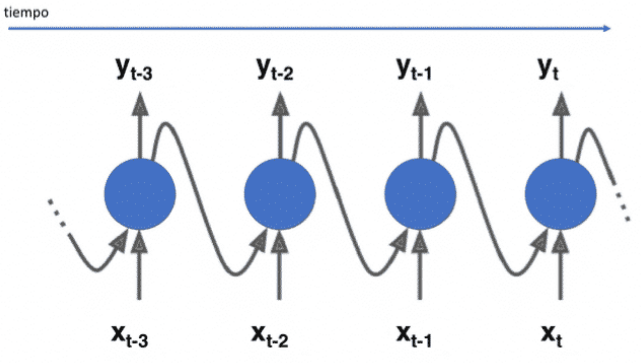
\includegraphics[scale=0.7]{RNN.PNG}  %Se incorpora imagen
    \caption{Redes Neuronales Recurrentes en el tiempo. Fuente: Torres, J (2019).}           %Titulo de la imagen
\end{figure}\\
Según se muestra en la figura 1, existen 4 neuronas interconectada a lo largo del tiempo, cada una de estas la entrada del nodo anterior, como también, su propia salida del instante de tiempo anterior para generar una salida. Llevándolo al problema de línea de embotellado, se utilizan los datos secuenciales a través del tiempo con las entradas que representarían la información recopilada de avisos y alarmas, las conexiones recurrentes son la retroalimentación y respuestas de salida a través del procesamiento de la información, los cuales actualizan el estado interno de la red para así, una vez que ha sido entrenado, pueda capturar patrones, estacionalidades y anomalías y así predecir procesos importantes de la línea. (Torres, J., 2019) \\ 
Sin embargo, es importante destacar que las RNN pueden ser computacionalmente intensivas, lo que significa que requieren recursos significativos de procesamiento y memoria para entrenarse y operar de manera eficiente, además que pueden ser afectadas por los \textit{"Exploding Gradients"} o \textit{"Vanishing gradients"} donde los valores de las gradientes para el entrenamiento es excesivamente alto (pendiente) por lo que se produce un error y detención en el proceso de aprendizaje. Dada la gran cantidad de datos con la que se cuenta es importante evaluar el impacto que estos proceso pueden traer a largo plazo a la eficacia del método. \\
Como antecedente que respalda y otorga valor a la utilización de esta metodología en el mantenimiento predictivo, se han encontrado estudios y tópicos que abordan la misma problemática en otros ámbitos, como por ejemplo, en la industria de la aviación. A partir del análisis lograron llegar a la siguiente conclusión, "Nuestros mejores modelos han sido capaces de detectar entre un 45-55\% de los casos anteriormente mencionados correctamente. Esta cifra debe contrastarse con el hecho de que no podemos asegurar que todos los fallos dentro de nuestro conjunto de datos tengan un
origen relacionado con los factores climatológicos estudiados. Por tanto, se ha cumplido
el objetivo: demostrar el potencial de predicción de estos datos aplicando Deep Learning." (López, J.M., 2021). Esto valida justamente que para el estudio de mantenimientos predictivos logra ser una herramiente de gran utilidad para abordarlo por Deep Learning mediante RNN.


\subsection{Métodos de Suavización Exponencial}
La suavización exponencial es un método de predicción propuesto durante 1950. En este caso las predicciones se llevan a cabo mediante una ponderación exponencial que decae a medida que las observaciones son más antiguas. De esta forma, los datos más relevantes para generar una mejor predicción son los más actuales. La mayor ventaja que tiene SES es que genera rápidamente un pronostico confiable, lo cual permite tomar, a su vez, decisiones tempranas. (Hyndman, R.J., \& Athanasopoulos, G., 2018)

\subsubsection{Método de Suavización Exponencial Simple (SES)}
Este método simple de suavización es utilizado para series de tiempo que no presentan tendencias claras o estacionalidades periódicas. Este utiliza un único parámetro de suavizado denominado "nivel" y actúa como un ponderador de los datos históricos. Gracias a su naturaleza exponencial tiene alto grado de precisión. (Vandeput, N., 2021)

Esta metodología puede ser extrapolada al problema de mantenimiento en la línea de embotellado y se identificaron las siguientes ventajas y desventajas. \\
\\
Por un lado, como fortalezas se observó que este método es altamente utilizado en el pronóstico de demanda destacándose en su fácil uso y eficiencia computacional, dando alertas tempranas para reducir el tiempo de inactividad. Además, su capacidad de actualización continua permite tomar decisiones en tiempo real. \\ 
\\
Por otro lado, las limitaciones de este modelo son su desempeño puede ser limitado con el uso de series temporales con patrones complejos o variaciones abruptas en los datos, como lo son las tendencias no lineales. Esto puede ser un gran problema ya que los datos históricos de la línea de embotellado presentaron más de 4 millones de observaciones. Además, el método hace como supuesto de que los datos históricos son relativamente estables, lo cual eso no siempre es verdad en la vida real y obviar esa información puede traer problemas a largo plazo, esto lo hace debido a que le da más peso a la información reciente dejando de lado la pasada. Agregando, no considera factores externos que pueden afectar el mantenimiento, como variaciones en la demanda del producto debido a distintas épocas del año o fluctuaciones en el suministro de materias primas. Por último, es de suma importancia la elección correcta de la constante inicial o "nivel" de suavizado. \\
\\
Como conclusión, este método puede ser efectivo como primer acercamiento a los datos pero no será sostenible en el tiempo debido a su simpleza, además que no es capaz de identificar las causas subyacentes de las fallas lo cual es esencial para otorgar retroalimentación e ir modificando los resultados a lo largo del tiempo. 

\subsubsection{Método Holt-Winters}
Este método es una adaptación a la metodología SES que genera predicciones más precisas cuando se trabaja son series de tiempo mayores, generando pronósticos a más largo plazo. Matemáticamente este utiliza una ecuación de pronóstico y tres ecuaciones de suavizado, las cuales van directamente relacionadas al nivel, tendencia y estacionalidad. De acuerdo a esta última característica, se consideran métodos aditivos cuando las variaciones estacionales son lo más similares a una constante, y métodos multiplicativos cuando las estacionalidades cambias proporcionalmente a lo largo de la serie de tiempo. (Hyndman, R.J., \& Athanasopoulos, G., 2018)
"El método Holt-Winters es una ampliación perfeccionada del enfoque de la suavización exponencial, mientras que el procedimiento de suavización proporciona una impresión general, movimientos a largo plazo en la información y permite la elaboración de pronósticos a corto plazo. Este método permite también el estudio de tendencia a futuro mediante la elaboración de pronósticos a mediano y largo plazo" (Mira, 2018). \\
\\
Este enfoque podría ser más efectivo que SES debido a su mayor complejidad, relacionándolo con la problemática en cuestión, se podría abordar de la siguiente manera. \\
\\
Como fortalezas, se identificó que igual que el método anterior, tiene una alta flexibilidad para adaptarse a distintos problemas y tipos de datos siendo adecuado para datos categóricos secuenciales que forman series de tiempo y presentan estacionalidades, lo cual como se puede ver en el estudio de los datos, hay patrones claramente definidos. Además, a partir de los parámetros del modelo se pueden extraer grandes interpretaciones de resultados con capacidad de tomar decisiones tempranas en el corto y largo plazo.  \\
\\
En las debilidades, de igual manera que el método SES, al ser metodologías de suavización no son capaces de actuar frente a cambios abruptos en el comportamiento de los datos, lo cual puede ser perjudicial a la hora del uso de la máquina en temporadas de altísima demanda. Agregando a lo anterior, las estimaciones de los parámetros es crucial para obtener predicciones certeras y esta a veces pueden ser a prueba y error lo cual no siempre es lo más eficiente. Por último, tampoco toma en cuenta los factores externos a la hora de la predicción, lo cual en un caso como este, es relativamente importante ya que en la realidad hay muchas variables exógenas que afectan el proceso por lo que deben ser controladas lo más que se pueda. \\



\subsection{Método de Croston y SBA}
El método de Croston "utiliza como base la atenuación exponencial simple separando la serie de tiempo" (Santa Cruz, Correa, 2017). Esto lo realiza en dos partes: una serie con valores positivos de demanda y una con los tiempos entre demandas consecutivas no nulas. En cada caso estima la predicción a través de una relajación y suavización exponencial con un mismo valor del parámetro de atenuación, para luego actualizar los valores en el momento en el que exista un valor no nulo de la demanda.\\
\\
El resultado de este método se ve expresado en términos de una tasa predictiva de demanda intermitente, con una razón entre demanda y el período en el que ocurre. De esta forma, la predicción obtenida para el próximo período es estimado a través de la razón entre estos dos valores.\\
\\
A pesar de que lograba demostrar un gran nivel de predicción en demanda intermitente, se demostró en su posterioridad que con ciertos valores del parámetro suavizante existía una desviación positiva. Ante esto, el método sufrió de una corrección derivándose al método SBA (Syntetos y Boylan), el que modifica el valor que multiplica la predicción de la demanda del período en ${(1-\alpha / 2)}$ para así ajustar la desviación proporcionada en la razón de los valores estipulados anteriormente.\\
\\
En el caso de plantear ambos métodos en el problema de la línea de embotellado, se puede concluir que el método de Croston muestra una ventaja en el manejo de datos intermitentes, siendo efectivo para tratar con series temporales que tienen una frecuencia de ocurrencia baja o discontinua, lo que es común en datos de fallas donde los eventos de falla no ocurren constantemente. Además su simplificación y adaptación del modelo, hace que sea fácil de implementar, pudiendo utilizarse para modelar diferentes patrones de ocurrencia de fallas, incluyendo fallas esporádicas, estacionales o aleatorias. Sin embargo, existe un sesgo en su predicción, tendiendo a generar predicciones hacia valores más altos, lo que puede llevar a una sobre estimación de la frecuencia de las fallas, sin contar la necesidad de ajustes, ya que requiere de parámetros específicos para diferentes conjuntos de datos, ni la falta de consideración de factores externos, donde se asume que los datos de ocurrencia de fallas son independientes de factores externos o variables de predicción adicionales, limitando los distintos escenarios.\\
\\
En el caso del método SBA, se observa que es eficiente para datos intermitentes, diseñado para lidiar con datos de demanda discontinua, irregular y esporádica. Además evita sesgos, debido a su ajuste, ayudando a evitar la sobre estimación de la demanda y proporciona pronósticos más reales, especialmente gracias a su adaptabilidad, ajustándose a diferentes patrones de intermitencia, incluyendo variaciones estacionales o aleatorias. Sin embargo, presenta una alta dependencia de parámetros, requiriendo la estimación de la tasa de ocurrencia de la demanda y tasa de interrupción de la demanda, siendo sensible al movimiento de datos y produciendo pronósticos inestables si no se maneja de forma adecuada.

\subsection{Fast Fourier Transform}
 %https://otexts.com/fpp2/decomposition.html
La transformada rápida de Fourier (FFT) es una técnica numérica que se utiliza para analizar señales en el dominio de la frecuencia a partir de datos en el dominio del tiempo. Permite descomponer una señal en sus componentes de frecuencia individuales, así entregando información sobre la amplitud y la fase de cada una. Luego se calcula la Transformada de Fourier de la señal en cuestión, convirtiéndola en una representación en el dominio de la frecuencia. En otras palabras, mostrando qué frecuencias están presentes en la señal y cuánta energía tienen. El resultado se le denomina "espectro de frecuencia", el que facilita la identificación de patrones y la toma de decisiones en aplicaciones de predicción y procesamiento de datos (Rao, Kim, Hwang, 2010).\\
\\
Es importante entender que este método es una técnica para analizar series de tiempo y señales para descomponer una señal en sus componentes de frecuencia. Aunque no es un método predictivo, se utiliza para extraer información relevante de las series temporales, lo que ayuda y es de utilidad en el proceso de pronóstico de fallas.\\
\\
Ante esto, al aplicarlo a la línea de embotellado, sirve para identificar patrones de frecuencia, detectando ciclos o patrones estacionales en los datos de fallas, así ayudando en la predicción de fallas recurrentes. Además, nos proporciona un análisis de componentes de frecuencia, determinando cuáles son las dominantes presentes en los datos y relevando información sobre características de los eventos repetitivos. Sin embargo, demuestra limitaciones en la detección de patrones no lineales, ya que se asume que los datos pueden descomponerse en componentes de frecuencia lineal, por ende, también tiene una alta dependencia de la calidad de los datos, donde si estos son incompletos los análisis pueden no ser confiables.


%\subsection{Transformada de Hilbert}
%La transformada de Hilbert conforma la señal con la mitad de la información en el dominio del tiempo y la otra mitad en el dominio de la frecuencia. Esta es equivalente a una rotación de 90° en la fase de cada componente armónica de la señal (https://www.osso.org.co/docu/tesis/2003/vibracion/D.pdf).
%Ver temas de teorías y análisis de señales y relacionar una señal a una serie de tiempo
%Colocar bien el métodod: terminar de ver estudio datos, ver correlaciones...
%...para esto queremos hacer esto debido a esto


\subsection{Comparación de metodologías}

Luego de analizar y comprender en profundidad cada una de las metodologías propuestas, teniendo en cuenta sus ventajas y desventajas, se puede concluir cual, o cuales, se adaptarían mejor al problema que se debe solucionar. Para cada una se explicó a priori la manera en que puede ser aplicada a este problema de predicción de mantenimiento, para llegar a una hipótesis sobre cual funcionaría mejor. Para el problema de mantenimiento predictivo en un entorno industrial, con un gran volumen de datos temporales, tanto la FFT como las RNN pueden ser opciones prometedoras. La FFT se enfoca en revelar patrones de frecuencia en señales complejas, mientras que las RNN se especializan en la captura de relaciones y patrones complejos en el historial de datos secuenciales y del comportamiento futuro de ellos. Por ahora se cuenta con la hipótesis de que ambas metodologías tienen el potencial de ofrecer predicciones precisas y exitosas para garantizar un funcionamiento óptimo en la producción botellas de vino.\\
\\
En contraste, los métodos de Suavización Exponencial y el Método de Croston, aunque pueden ser útiles en varios contextos de pronóstico, se cree por ahora que no serian tan adecuados en comparación a los otros dos propuestos, para abordar la complejidad y tamaño de nuestras bases de datos. Estos métodos funcionan mejor con series de tiempo más simples y regulares, mientras que el entorno en cuestión presenta múltiples factores y variables tanto endógenas como exógenas a analizar. 





\section{Análisis de datos}

En el proceso de análisis de datos, además de realizar una observación general de las bases de datos, se consideró esencial la creación de gráficos que representaran de manera visual la relación entre diversos parámetros seleccionados. Esto permitió obtener una comprensión más clara y dinámica de cómo se comportan los datos a lo largo del tiempo, y facilitó la identificación de patrones y tendencias.

\subsection{Frecuencia}
Para adentrarnos en este análisis, optamos por confeccionar gráficos de frecuencia que representaran la cantidad de ocurrencia de las distintas alarmas y avisos. Este corresponde a una visión general de los datos ya que se cuenta la ocurrencia de las alarmas y avisos correspondientemente en todo el periodo de tiempo de análisis. Este enfoque nos permitió identificar cuáles de estos eventos eran más recurrentes a lo largo de la serie temporal. Dado que nuestro objetivo principal implica la creación de un modelo predictivo, es necesario contar con una amplia cantidad de datos para comprender el comportamiento de la máquina en cuestión. En consecuencia, decidimos iniciar nuestro análisis enfocándonos en los eventos más recurrentes en nuestra base de datos, ya que son estos los que aportan una mayor cantidad de información.\\

\begin{figure}[H]
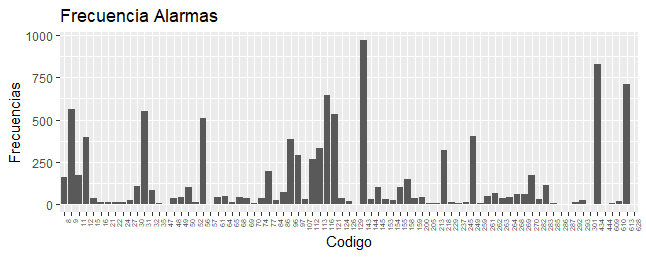
\includegraphics[width=0.8\textwidth]{Graficos/FrecuenciaAlarmas.png}
  \caption{Frecuencias de cada alarma.}
\end{figure}

Del gráfico se distingue claramente que existen 3 tipos de alarmas las cuales poseen una mayor frecuencia estas son las siguientes: Falta cera en botella, Avería sonda presión sondra y Volante no en reposo, con las frecuencias correspondientes a 971, 829 y 713 ocurrencias respectivamente. Además, se observa que existe una gran cantidad de alarmas que su ocurrencia esta muy por debajo de las 250 ocurrencias, aún más especifico 18 tipos de alarma no poseen más de 10 ocurrencias en la totalidad del periodo de análisis.\\

\begin{figure}[H]
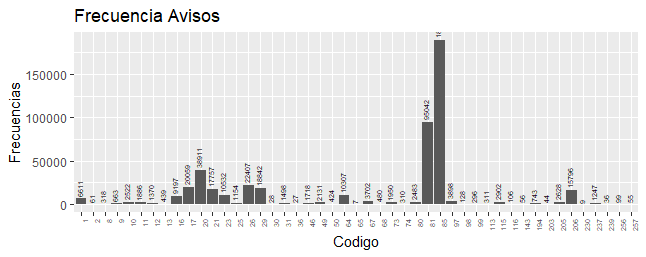
\includegraphics[width=0.8\textwidth]{Graficos/FrecuenciaAvisos.png}
  \caption{Frecuencias de cada aviso.}
\end{figure}

A primera vista se puede ver como las frecuencias de los avisos se disparan en comparación a la ocurrencia de las alarmas alcanzando valores por sobre los 1000 en más del 50\% de los tipos de alarmas, específicamente en 28 tipos de 49. Los 3 tipos mas recurrentes de avisos son Control automático ventilador campana, Modulación entrada producto equivocada y Señal bloqueo botellas activada en linea con una frecuencia de 189181, 95042 y 38911 respectivamente.

Como se observo de los gráficos anteriores, la frecuencia de los avisos es superior a la de las alarmas en gran medida. Con el objetivo de visualizar la relación entre la cantidad de alarmas y avisos totales en el tiempo se realizo el siguiente gráfico: 

\begin{figure}[H]
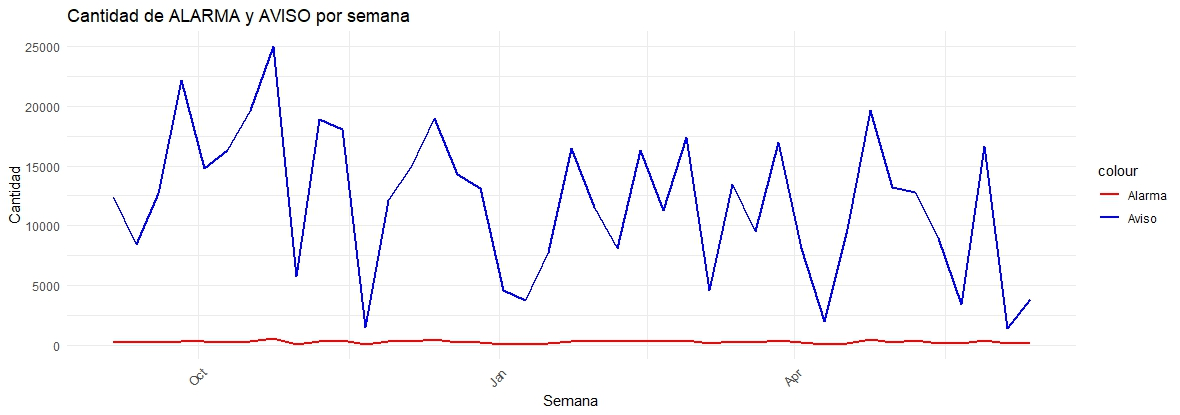
\includegraphics[width=1.1\textwidth]{Graficos/Avisos_Alarmas_semana.jpeg}
\caption{Cantidad de avisos y alarmas por semana.}
\end{figure}

Este gráfico demuestra que en todo el periodo de tiempo la cantidad de avisos es superior a la de alarmas. Además, por el nivel de detalle alcanzado para los avisos se ven grandes fluctuaciones en periodos del tiempo identificados que es interesante analizar. 

Del análisis de frecuencia quedan instancias de análisis abiertas como es ver la relación de las alzas y descensos de cantidad de avisos en un instante de tiempo con la realización de una mantención. Por otro lado, si bien es importante ver cuales son los eventos más frecuentes se debe estudiar el tipo de alarma de menor frecuencia en relación a los ritmos de producción ya que se puede dar el caso donde una alarma o aviso es de gran gravedad y altera inmediatamente el proceso productivo. 

\subsection{Avisos y Alarmas}
Para continuar con nuestro análisis, una vez teniendo en cuenta cuales eran los eventos más recurrentes, tanto para las alarmas como para los avisos, decidimos verificar como se comportaba cada uno de los 10 eventos con mayor frecuencia en ambas categorías a lo largo de la serie de tiempo, para verificar como este se conecta con las fechas de mantenciones, y así verificar si este evento afecta de alguna manera la producción en la linea de embotellamiento.
\\
\begin{figure}[H]
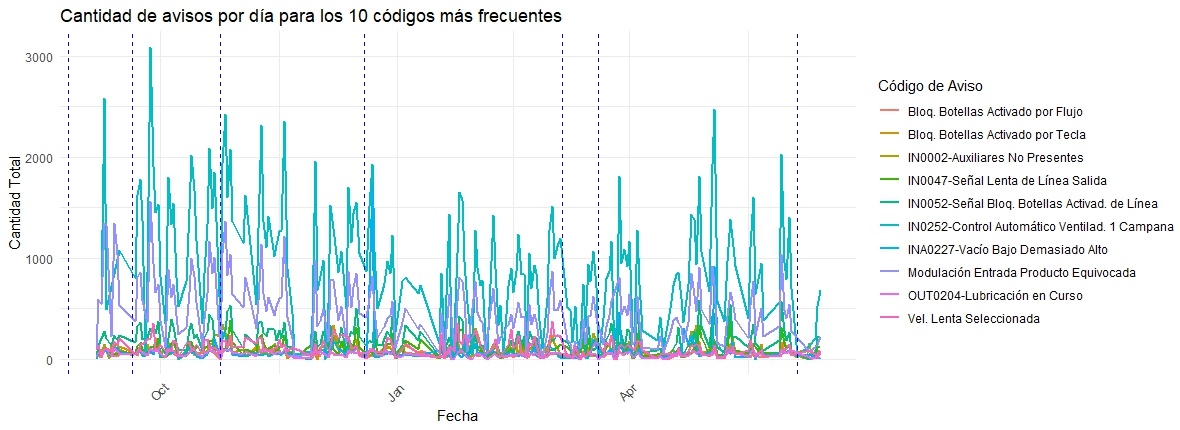
\includegraphics[width=1.1\textwidth]{Graficos/AVISOS_MANTENCIONES_FINAL_TOP10.jpeg}
\caption{cantidad de avisos por día para los 10 mas frecuentes y mantenciones.}
\end{figure}


Como podemos observar en el gráfico anterior, dentro de los avisos mas recurrentes, se pueden identificar diversos comportamientos, por una parte tenemos eventos que no parecen tener algún tipo de correlación con la cercanía al momento de una mantención (lineas punteadas verticales) como podrían ser los aviso cambio de velocidad en la maquina o de bloqueos automáticos, esto se puede deber a que son avisos que no perjudican el funcionamiento de la maquina. Por otro lado podemos observar que hay avisos cuya frecuencia tiene un grado de correlación con la cercanía de las mantenciones, esto lo podemos ver en la frecuencia de estos avisos, por ejemplo si observamos el aviso que tiene la mayor frecuencia durante la gran parte del tiempo, el aviso cuya descripción es control automático ventilador, vemos que cuando se acerca la mantención la frecuencia de este tiende a dispararse, pero luego de la mantención esta frecuencia tiene una bajada considerable, esto puede significar que este aviso es un factor de alerta de una falla, si es que el mantenimiento cercano es correctivo.


\begin{figure}[H]
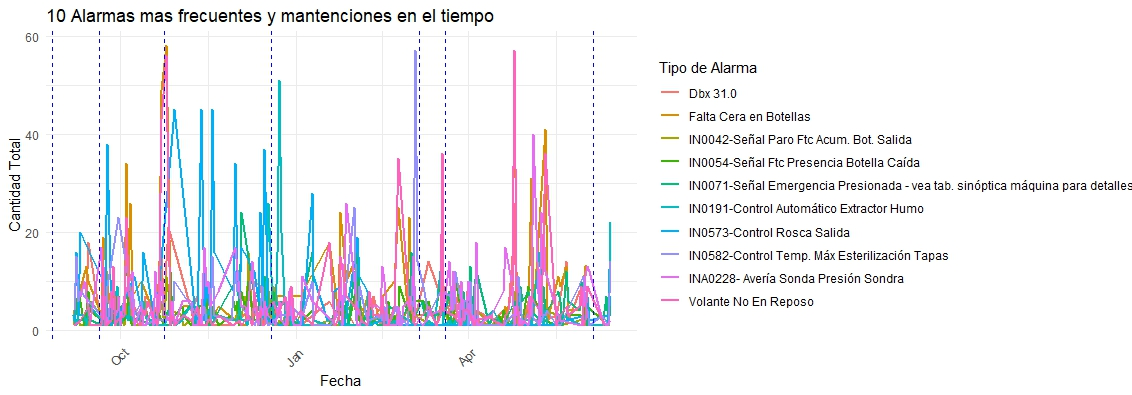
\includegraphics[width=1.1\textwidth]{Graficos/ALARMAS_MAS_FRECUENTES_TOP10 (1).jpeg}
\caption{cantidad de alarmas por día para las 10 mas frecuentes y mantenciones.}
\end{figure}





Al ver el gráfico anterior, podemos darnos cuenta que dentro de las alarmas mas recurrentes, podemos encontrar diferentes comportamientos con respecto a las fechas de las mantenciones. Dentro de los grupos de comportamiento observamos que hay alarmas cuya frecuencia tiene algún tipo de correlación con cuando se realiza la mantención, es decir, cuando se avecina una mantención su frecuencia se dispara y luego de la mantención esta frecuencia se desploma. Por otro lado, podemos observar que hay grupos de alarmas cuya frecuencia es independiente de la presencia de una mantención. El comportamiento de una tipo de alarma en concreto previo a una mantención es de gran utilidad, porque nos permite verificar si se realizó mantenimiento correctivo o preventivo, una vez sabiendo que tipo de mantenimiento es podemos clasificar el tipo de alarma como un posible factor que puede producir una falla.\\

Para continuar con la linea de análisis anterior, se graficó la cantidad de alarmas totales por día, esto con el objetivo de corroborar el comportamiento que se estaba analizando a nivel particular de cada una de las alarmas a nivel general, viendo su correspondencia con las mantenciones, las cuales son identificadas por lineas verticales en los gráficos. 
\\
\begin{figure}[H]
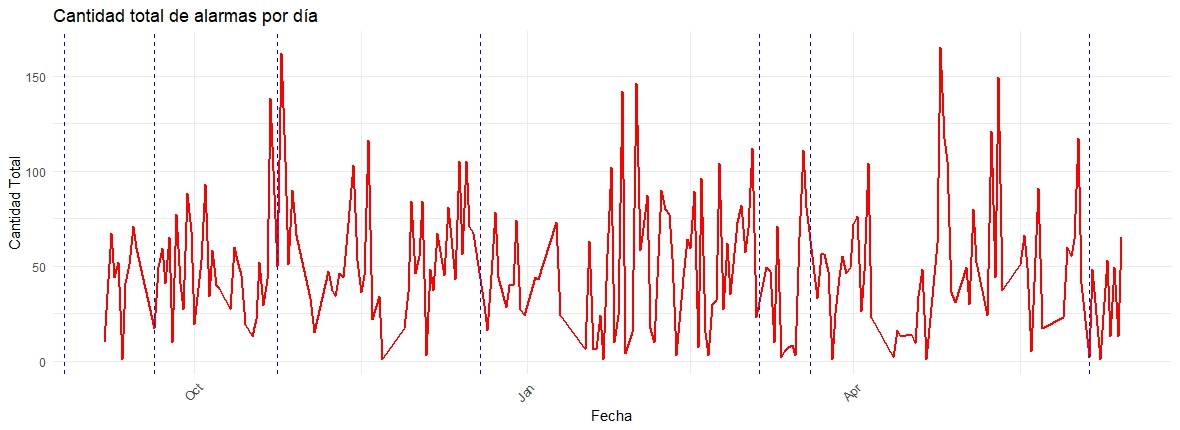
\includegraphics[width=1.1\textwidth]{Graficos/Alarmas_mantenciones_diario.jpeg}
\caption{Cantidad de alarmas por día y mantenciones realizadas.}
\end{figure}




Si bien en algunas mantenciones se logra el comportamiento que esperábamos el cual por nuestra definición de falla es que previo a una mantención la cantidad de alarmas es grande frente a la cantidad posterior debido a que en la mantención se soluciona la falla, también se observa que este comportamiento ocurre justo antes o después de la mantención dando lugar a analizar un desfase de los resultados de la mantención como también de buscar las causas de cada una de las fluctuaciones, por lo que es mas concluyente medir el comportamiento a nivel individual. 


\subsection{Producción}

\begin{figure}[H]
\includegraphics[width=0.9\textwidth]{Graficos/ProducciónAcumulada.jpeg}
\caption{Producción de botellas de vino acumuladas y mantenciones.}
\end{figure}


Este gráfico muestra la cantidad de botellas acumuladas en el periodo de tiempo, en su generalidad el crecimiento es estable, pero se pueden identificar pendientes que dejan en evidencia la presencia de inestabilidades interesantes de analizar. Por una parte si observamos en el medio podemos ver una pendiente muy positiva, lo que significa gran volumen de producción en poco tiempo. Una observación que podría haber sido alarmante es una pendiente negativa o paralela, mostrando problemas en la producción. También la información de producción entregada, a pesar de ser difícil de manejar dada su cantidad de valores, se agrupo por día para simplificar. Las lineas verticales de color rojo muestran las mantenciones realizadas a la maquina, luego de realizar este cruce nos damos cuenta la importancia de generar una mayor análisis entre producción, integrando variables de alertas y alarmas que impliquen una correlación y causalidad con la producción de manera que permitan predecir una probabilidad de falla en un futuro.
%falta analisis grafico

\subsection{Relaciones extraídas}

El comportamiento que se buscaba estudiar con los gráficos anteriores es la relación entre avisos, alarmas y producción con las mantenciones. Como fue descrito anteriormente nuestra hipótesis de falla, se basa en una aviso o alarma que repentinamente a lo largo de la serie de tiempo tiene una alza considerable en frecuencia antes de una mantención, y posterior a esta, su frecuencia baja en gran medida, como mencionamos anteriormente actualmente se realizan dos tipos de mantenciones, en primer lugar correctivas, las cuales se realizan al luego de que ocurra una falla para arreglar la maquina y por otro lado encontramos mantenciones preventivas las cuales se hacen cada cierto tiempo. Nuestra hipótesis de falla se base en el primer tipo de estas mantenciones, una vez identifiquemos cuales son las alarmas o los avisos cuya frecuencia se comporta de la forma anterior, entonces podremos identificar claramente una falla, y teniendo este dato. Tendremos dejar una frecuencia limite para estos eventos diaria, la cual si se alcanza se debe realizar un mantenimiento. %me hace sentido, pero voy a comer y vuelvo 



\section{Futuro}

\subsection{Metodología}

La recopilación de información junto al análisis de datos que se ha desarrollado a la fecha nos permite definir una linea de acción futura o metodología para la búsqueda de una solución a la problemática. Esta se separa en 2 grandes grupos el estudio y la predicción:
 

\subsubsection{Estudio}
Actualmente nos encontramos en esta etapa, donde el foco principal es el entendimiento de los datos. Aquí se busca que el descubrimiento de los datos converja a la elección de un método de resolución, para esto las actividades a seguir son:
\begin{enumerate}
\item Trasformar los datos a series de tiempo
\item Clusterizar avisos y alarmas
\item Identificar paradas de máquina
\item Determinar correlaciones del análisis gráfico
\item Evaluar correlaciones con herramientas estadísticas 
\end{enumerate}

\subsubsection{Predicción}
Esta macro etapa se encarga de la elaboración del modelo de solución. La cual se descompone en las siguientes subb etapas:
\begin{enumerate}
\item Generar dashboard de control
\item Testear métodos 
\item Definir modelo 
\item Entrenar al modelo
\item Validar resultados del modelo
\item Proponer una política de decisión de mantenimiento
\item Determinar el peso de la variable sobre la predicción de las fallas
\item Generar un código que indique al probabilidad de falla

\end{enumerate}

\subsection{Desglose de la predicción}

Respecto al uso de los datos, los cuales fueron entregados por el equipo docente se tomaron consideraciones para la utilización y manejo, así evitar sobreajuste y mejorar la precisión del modelo. Es por esto que se eligió utilizar el principio denominado 50/25/25, la cual es una regla comúnmente utilizada en la predicción y validación de modelos predictivos. Esta regla se caracteriza por el desglose de los datos en 3 grupos, el conjunto de entrenamiento, el conjunto de validación y finalmente el conjunto de prueba (Nieves, 2016).
%Es un modelo determinístico y no lineal -> sistema caótico
%Para evitar overfiting, se dividen los datos en tres grupo, trabajando con el primer 50% para luego analizar y pretestear con el siguiente 25% para finalmente predicir el ultimo 25% y finalmente compararlo con nuestros datos -> para entrenar redes neuronales y en caso de simulaciones
\subsubsection{Entrenamiento del modelo}

En un principio se trabaja solo con el $50\%$ de todos los datos, estos se utilizan para la creación y entrenamiento del modelo, cabe mencionar que mientras mayor sea este conjunto de datos el modelo es posible que el modelo tengo un mejor rendimiento. 

\subsubsection{Validación del modelo}
Luego de la creación y entrenamiento del modelo, se utiliza el modelo generado con el conjunto de datos del principio, y se agrega el siguiente $25\%$ de los datos los cuales se utilizan para la validación, evaluando el rendimiento y optimizar su funcionamiento.

\subsubsection{Prueba del modelo}
 Finalmente el ultimo $25\%$ de los datos es el conjunto que se conoce como conjunto de prueba, después de que se haya seleccionado y ajustado el conjunto de validación. Este conjunto proporciona una estimación imparcial de como se desempeñaría el modelo en datos ante datos desconocidos.
 
\subsection{Carta Gantt}
Se llevó a cabo una carta Gantt (Anexo) lo cual tiene como propósito ser una herramienta fundamental para la gestión del proyecto, trazando una línea base para que todo el equipo sepa cuales son los objetivos esperados y cómo se debe ir trabajando. Se usó para generar dependencias entre tareas, definir importancia y tiempo estimado para su realización. En específico, para la entrega 1, se cumplieron las tareas propuestas según el calendario, no dejando de lado la ruta crítica, como por ejemplo, el estudio de la literatura y metodología, exploración de datos, caso base y presentación 1. Para la siguiente entrega, se espera tener un análisis mas exhaustivo de los datos, implementación simplificada de la metodología y propuesta de política y trabajo.

\section{Conclusiones}

A modo de síntesis, el cambio de enfoque de mantenimiento, pasando de uno preventivo/correctivo a uno predictivo, representa un avance significativo hacia la mejora de las operaciones en la línea de embotellamiento de la empresa vitivinícola en cuestión. Este cambio significaría un aumento considerable en la eficiencia operativa, disminución de detenciones innecesarias, gracias a la optimización de la gestión del mantenimiento, permitiendo cumplir de mejor manera el objetivo de satisfacer la demanda de manera más efectiva.\\
\\
El análisis de las bases de datos, que abarcan un periodo de 20 meses y más de 4 millones de observaciones, ha sido esencial en este proceso. Mediante la definición de metas y la identificación de indicadores de desempeño, se encontró el camino para evaluar el desempeño de los modelos predictivos que se desarrollen. Además, la aplicación del principio 50/25/25 para dividir los datos en conjuntos de entrenamiento, validación y prueba, se espera que sea una estrategia efectiva para demostrar y asegurar la solidez de los modelos, y así poder encontrar el que mejor se adapte al problema. Sin embargo es importante recalcar la posible influencia de variables externas en el problema, las cuales pueden llegar a influir en la producción y en las fallas.\\
\\
El análisis de literatura sobre diversas metodologías, que incluyen redes neuronales recurrentes, métodos de suavización exponencial, el método Holt-Winter, el método de Croston, y el enfoque de SBA y Fast Fourier Transform, nos han brindado una comprensión profunda de cada enfoque en el contexto específico del problema a resolver en nuestra línea de embotellamiento. Entre estas metodologías, se espera que RNN y FFT se adapten de mejor manera al problema, gracias a la capacidad que tienen de trabajar grandes volúmenes de datos variados. \\
\\
En resumen, en esta primera etapa, ya se cuenta con un avance significativo, gracias al análisis del caso base e investigación de posibles metodologías, hacia la implementación del mantenimiento predictivo en nuestra empresa vitivinícola, sino que también establece las bases para una gestión más eficiente y rentable de nuestros recursos de mantenimiento. Esto, en última instancia, contribuirá a mejorar nuestra competitividad y nuestro éxito continuo en el mercado vinícola, logrando generar una herramienta de utilidad para la empresa asesorada.

\newpage
\section{Referencias Bibliográficas}
%https://www-webofscience-com.pucdechile.idm.oclc.org/wos/woscc/full-record/WOS:000474741700049

Bonet Cruz, I., Salazar Martínez, S., Rodríguez Abed, A., Grau Ábalo, R., $\&$ García Lorenzo, M. M. (2007). Redes neuronales recurrentes para el análisis de secuencias. \textit{Revista Cubana de Ciencias Informáticas} 1(4), 48-57. Recuperado de: \href{https://www.redalyc.org/pdf/3783/378343634004.pdf}{https://www.redalyc.org/pdf/3783/378343634004.pdf} \\

Hyndman, R.J., $\&$ Athanasopoulos, G. (2018) Forecasting: principles and practice, 2nd edition, \textit{OTexts: Melbourne, Australia.} \href{https://otexts.com/fpp2/expsmooth.html}{https://otexts.com/fpp2/expsmooth.html} \href{https://otexts.com/fpp2/holt-winters.html}{https://otexts.com/fpp2/holt-winters.html}\\

Nieves, D. ¿Qué es el escenario de entrenamiento, validación y prueba de conjuntos de datos en aprendizaje automático?. Recuoerado de: \href{https://es.quora.com/En-el-aprendizaje-autom%C3%A1tico-cu%C3%A1l-es-el-prop%C3%B3sito-de-dividir-los-datos-en-conjuntos-de-prueba-y-conjuntos-de-entrenamiento}{https://es.quora.com/En-el-aprendizaje-automitco}\\

Mira Segura, L. L., Trejo Martínez, A., $\&$ López Cruz, D. (2018). \textit{Aplicación de Holt-Winters para pronósticos de inventarios.} CIENCIA UANL, 21(90). DOI: \href{https://doi.org/10.29105/cienciauanl21.90-2}{https://doi.org/10.29105/cienciauanl21.90-2} \\

López Camuñas, J. M. (2021). Predictive Maintenance Using Deep Learning. Tesis de grado, Grau d'Enginyeria Informàtica, Facultat de Matemàtiques i Informàtica, Universitat de Barcelona. Recuperado de: \href{https://diposit.ub.edu/dspace/bitstream/2445/182392/3/tfg_jose_manuel_lopez_camu%C3%B1as.pdf}{https://diposit.ub.edu/dspace/bitstream/2445/182392/3/tfg_jose_manuel_lopez_camu} \\

Pérez Ortiz, J. A. (2002). Modelos predictivos basados en redes neuronales recurrentes de tiempo discreto. \textit{Tesis doctoral, Universidad de Alicante} Recuperado de: 
\href{https://www.dlsi.ua.es/~japerez/pub/pdf/tesi2002.pdf}{https://www.dlsi.ua.es/~japerez/pub/pdf/tesi2002.pdf} \\


Rao, K. R., Kim, D. N., $\&$ Hwang, J.-J. (2010). \textit{Fast Fourier Transform - Algorithms and Applications.} Springer Dordrecht. DOI: \href{https://doi.org/10.1007/978-1-4020-6629-0}{https://doi.org/10.1007/978-1-4020-6629-0} \\ 

Santa Cruz, R. $\&$ Correa, C. (2017). Previsión de demanda intermitente con métodos de series de tiempo y redes neuronales artificiales: Estudio de caso. DOI: \href{https://doi.org/10.15446/dyna.v84n203.63141}{https://doi.org/10.15446/dyna.v84n203.63141} \\

Torres, J. (2019). Redes Neuronales Recurrentes. Recuperado de: \href{https://torres.ai/redes-neuronales-recurrentes/}{https://torres.ai/redes-neuronales-recurrentes/} \\

Vandeput, N. (2021). Data Science for Supply Chain Forecasting (2nd ed.). \textit{De Gruyter.} Recuperado de: \href{https://towardsdatascience.com/simple-exponential-smoothing-749fc5631bed}{https://towardsdatascience.com/simple-exponential-smoothing-749fc5631bed}






\newpage
\section{Anexos}
\subsection{Carta Gantt:}
Para ver la Carta Gantt se debe presionar \href{https://uccl0-my.sharepoint.com/:x:/r/personal/mtago_uc_cl/_layouts/15/Doc.aspx?sourcedoc=%7BBBFA9B63-7895-461D-AF00-714DC960626F%7D&file=Carta%20Gantt.xlsx&action=default&mobileredirect=true}{aquí}.
\subsection{Anexo 1:}
\begin{table}[!ht]
    \centering
    \begin{tabular}{|l|l|}
    \hline
        Codigo & Descripción \\ \hline
        0 & no asignado \\ \hline
        8 & IN0070-Señal Bloqueo Inversor Motor Principal \\ \hline
        9 & IN0071-Señal Emergencia Presionada - vea tab. sinóptica máquina \\ \hline
        11 & IN0086-Control Sobretemperatura Armario \\ \hline
        12 & IN0042-Señal Paro Ftc Acum. Bot. Salida \\ \hline
        15 & IN0096-Control Automático Alimentación Ctrl Nivel/Tapa \\ \hline
        16 & IN0081-Control Presostato No Hay Aire en Red \\ \hline
        21 & Error Acoplamiento Tapadora 2 \\ \hline
        22 & Temperatura Máx. Cuba Bombas \\ \hline
        24 & Conteo Botellas Alcanzado \\ \hline
        27 & Mantenimiento Programado \\ \hline
        30 & Error Acoplam. Enjuagadora \\ \hline
        31 & IN0054-Señal Ftc Presencia Botella Caí­da \\ \hline
        32 & IN0064-Señal Mesa Acum. Bot. Llena \\ \hline
        35 & IN0064-Señal Mesa Acum. Bot. Llena \\ \hline
        47 & Control Seguridades \\ \hline
        48 & IN0034-Control Disp. Automáticos Intervenidos Grave \\ \hline
        49 & IN0170-Control Estrella Entrada \\ \hline
        50 & IN0171-Control Estrella Salida \\ \hline
        52 & IN0173-Control Rosca Salida \\ \hline
        56 & IN0191-Control Automático Extractor Humo \\ \hline
        57 & IN0180-Control Presostato Tratamiento 1 \\ \hline
        61 & IN0195-Control Auto. Motor Ventilador 1 Campana Enjuagadora \\ \hline
        64 & IN0196-Control Presostato Correa Ventilador 1 Campana Enjuagadora \\ \hline
        65 & IN0270-Control Estrella Entrada \\ \hline
        68 & IN0273-Control Rosca Salida \\ \hline
        69 & IN0277-Control Botella Colgada \\ \hline
        70 & IN0294-Control Auto. Bomba Vacío Alto \\ \hline
        74 & IN0280-Control Cuba Alcohol Desalineada \\ \hline
        77 & Falta Comunicación PLC Depósito \\ \hline
        84 & IN0250-Control Presostato Atascamiento Filtro 1 Campana \\ \hline
        86 & PLC Parado \\ \hline
        96 & IN0241-Control Presostato Correa Ventilad. 2 Campana \\ \hline
        97 & IN0470-Control Estrella Entrada \\ \hline
        107 & IN0454-Control Canal Falta Tapas Pieza Final Paro Máquina \\ \hline
        112 & IN0467-Control Temperatura No Adec.  Pistola Pegamen. \\ \hline
        113 & IN0570-Control Estrella Entrada \\ \hline
        116 & IN0573-Control Rosca Salida \\ \hline
        121 & IN0582-Control Temp. Máx Esterilización Tapas \\ \hline
        124 & IN0577-Control Botella Colgada \\ \hline
        
    \end{tabular}
    \caption{Alarmas y sus descripciones parte 1}
\end{table}

\begin{table}[!ht]
    \centering
    \begin{tabular}{|l|l|}
    \hline
    Codigo & Descripción \\ \hline
    126 & IN0592-Control Auto. Termorresistent. Esterlización Tapas \\ \hline
        129 & Botella Rota TV \\ \hline
        143 & Falta Cera en Botellas \\ \hline
        144 & Faltan Corchos en Botellas \\ \hline
        145 & Error Codif. Torreta \\ \hline
        153 & IN0546-Control Guía Entrada acción. \\ \hline
        154 & IN0560-Control Patí­n Gas/Vacío Pos. Trab. \\ \hline
        155 & IN0517-Control Caja Compresión Abierta \\ \hline
        158 & Alimentador Tapones Vacío \\ \hline
        159 & Botella Ausente \\ \hline
        200 & IN0246-Control Guía Entrada Accion. \\ \hline
        205 & IN0305-Control Botella Explotada Salida \\ \hline
        213 & IN0186-Control Presostato Soplado Gotas \\ \hline
        218 & Dbx 27.1 \\ \hline
        229 & IN0950-Control Alarma Ups \\ \hline
        237 & INA0000-Falta Ref. Velocidad de Inversor Motor Principal \\ \hline
      245 & IN0484-Control Bloq. Inversor Motor Cabezales  \\ \hline
        249 & Dbx 31.0 \\ \hline
        259 & IN0954-Control Automáticos Circuitos 480V CA Drive \\ \hline
        261 & Master \\ \hline
        262 & Enjuagadora \\ \hline
        263 & Llenadora \\ \hline
        264 & Tapadora Rosca \\ \hline
        268 & Rosca \\ \hline
        269 & Estrellas Enjuagadora \\ \hline
        270 & Estrellas Llenadora \\ \hline
        282 & Dbx 35.1 \\ \hline
        283 & INA0322-Control Seguridad Cubeta \\ \hline
        285 & IN0320-IN0321-Leva Desc. Conos Delanteros Desalin. \\ \hline
        286 & IN0230-IN0231-Leva Desc. Conos Recipient. Desalin. \\ \hline
        287 & IN0230-IN0231-Leva Desc. Conos Recipient. Desalin. \\ \hline
        292 & IN0234-Control Posición Pirómetro \\ \hline
        293 & INA0227-Avería Sonda Presión Circuito Vací­o Bajo \\ \hline
        301 & IN0377- Ajuste Auto. Anillo Dispositivos \\ \hline
        434 & INA0228- Averí­a Sonda Presión Sondra \\ \hline
        444 & Generic Cause CG \\ \hline
        609 & Timeout Solicitado \\ \hline
        610 & Timeout Fase \\ \hline
        613 & Volante No En Reposo \\ \hline
        628 & Temperatura No Mantenida \\ \hline
    \end{tabular}
     \caption{Alarmas y sus descripciones parte 2}
\end{table}


\newpage
\subsection{Anexo 2}
\begin{table}[!ht]
    \centering
    \begin{tabular}{|l|l|}
    \hline
        Código & Descripción \\ \hline
        0 & No Asigando \\ \hline
        1 & IN0083-Selector Panel de Mando Volante Habilitado \\ \hline
        2 & IN0081-Control Presostato No Hay Aire en Red \\ \hline
        8 & Elevación en Curso \\ \hline
        9 & IN0000-Rotación Solicitado \\ \hline
        10 & IN0040-Señal Ftc Lenta Ninguna Botella Entrada \\ \hline
        11 & IN0041-Señal Ftc Paro Ninguna  Botella Entrada \\ \hline
        12 & IN0042-Señal Paro Ftc Acum. Bot. Salida \\ \hline
        13 & Señal Ftc Lenta Acum. Bot. Salida \\ \hline
        16 & IN0046-Señal Paro de  Lí­nea Salida \\ \hline
        17 & IN0047-Señal Lenta de Lí­nea Salida \\ \hline
        20 & IN0052-Señal Bloq. Botellas Activad. de Línea \\ \hline
        21 & Bloq. Botellas Activado por Tecla \\ \hline
        23 & Bloq. Botellas Activado por Flujo \\ \hline
        25 & IN0031-Grasa Bloqueada \\ \hline
        26 & Vel. Lenta Seleccionada \\ \hline
        29 & IN0002-Auxiliares No Presentes \\ \hline
        30 & IN0061-Control Presostato No Gas Inerte \\ \hline
        31 & OUT0031-Mando Disposit. Engrase \\ \hline
        36 & CIP-Señal de CIP de Alarma \\ \hline
        46 & Puertas Desbloq. \\ \hline
        49 & IN0174-Control Protecciones Delanteras Abiertas \\ \hline
        50 & IN0175-Control Protecciones Traseras Abiertas \\ \hline
        64 & OUT0204-Lubricación en Curso \\ \hline
        65 & IN0291-Control Auto. Motor Ajuste Depósito \\ \hline
        67 & IN0274-Control Protecciones Delanteras Abiertas \\ \hline
        68 & IN0275-Control Protecciones Traseras Abiertas \\ \hline
        73 & INA0200-Nivel Má­nimo Depósito \\ \hline
        74 & INA0200-Nivel Máximo Depósito \\ \hline
        80 & Primer Llenado en Curso \\ \hline
        81 & Modulación Entrada Producto Equivocada \\ \hline
        85 & IN0252-Control Automático Ventilad. 1 Campana \\ \hline
        97 & IN0474-Control Protecciones Delanteras Abiertas \\ \hline
        98 & IN0475-Control Protecciones Traseras Abiertas \\ \hline
        99 & IN0476-Control Protecciones Laterales Abiertas \\ \hline
        113 & IN0594-Control Auto. Motor Ajuste Émbolos \\ \hline
        115 & IN0574-Control Protecciones Delanteras Abiertas \\ \hline
        116 & IN0575-Control Protecciones Traseras Abiertas \\ \hline
        143 & Faltan Corchos en Botellas \\ \hline
        194 & OUT0210-Válvula Entrada Producto Cerrada por Falta \\ \hline
        203 & OUT0207-Presión Cilindros Demasiado Baja \\ \hline
        205 & INA0227-Vacío Bajo Demasiado Bajo \\ \hline
        206 & INA0227-Vacío Bajo Demasiado Alto \\ \hline
        230 & IN0951-Control Ups Funcionamiento de Batería \\ \hline
        237 & Señal Falta Solicitud lista de CIP \\ \hline
        239 & Mando Manual Habilitado \\ \hline
        256 & Máquina ligeramente Desfasada \\ \hline
        257 & Máquina Desfasada \\ \hline
    \end{tabular}
     \caption{Avisos y sus descripciones}
\end{table}
\end{document}

